
% ════════════════════════════════════════════
% 模型准备（5.1.2.模型准备.tex，三级子块）
% ════════════════════════════════════════════
\subsubsection{模型准备}

\textbf{1.数据预处理}

附件一给出了某一天不同时刻的电价、小区负载和光伏发电预测功率，时间分辨率均为 10 分钟，其中末行时间记作 $0{:}00{+}1$，表示当天 24:00。原始数据以时间字符串索引，无法直接用于逐时段递推计算，因此需要先进行时间对齐与数值化处理。为便于后续建模，首先对数据进行预处理，具体步骤如下。

将一天划分为 144 个等长时间间隔，第 $k$ 个间隔对应时段 $[k\Delta t,(k+1)\Delta t]$，其中 $\Delta t=1/6$ 小时。设第 $k$ 个间隔的负载功率为 $L_k$、光伏功率为 $S_k$、电价为 $p_k$，则数据点 $(k+1)\Delta t$ 处记录的功率值即为该间隔内的平均功率，其能量可表示为：
\begin{equation}
    E_k = P_k\,\Delta t,\quad k=0,1,\dots,143
\end{equation}
其中，$E_k$ 表示第 $k$ 个间隔的能量（kWh），$P_k$ 为该间隔的功率（kW）。将时间边界 $0{:}00{+}1$ 映射为 24:00，并对三列数据统一执行数值化与缺失检查，预处理前后对比如图\ref{fig:preprocess1}所示。

\begin{figure}[H]
    \centering
    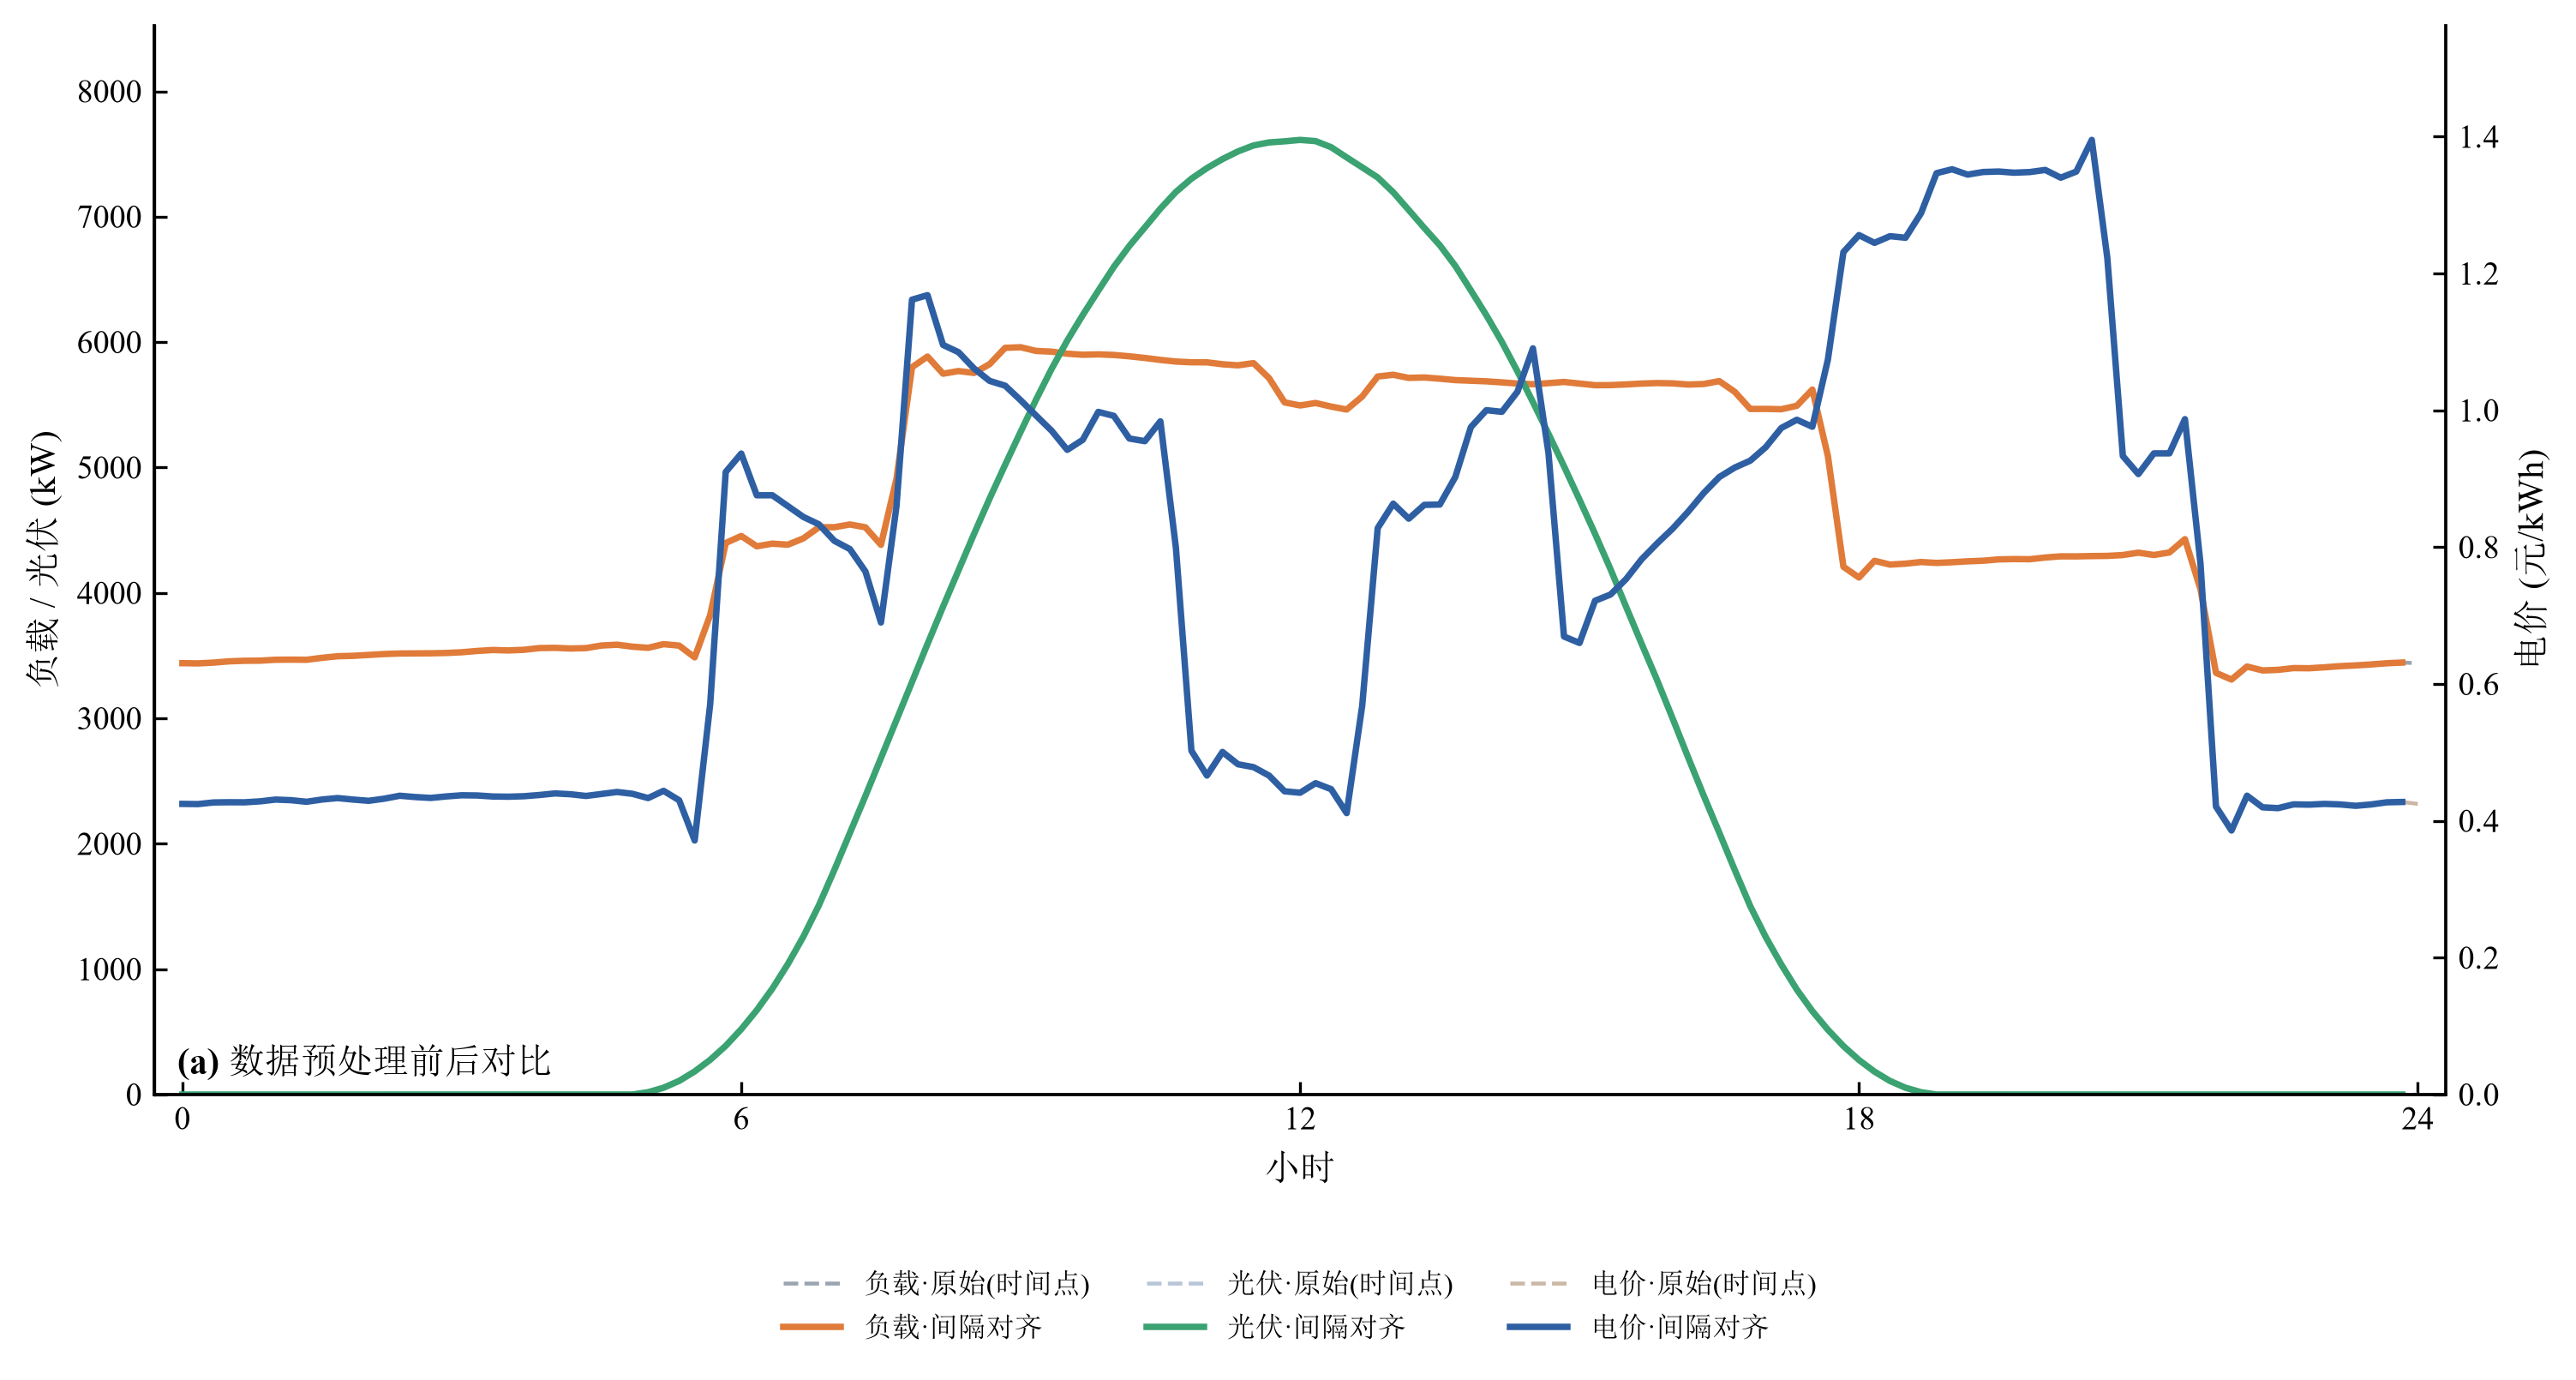
\includegraphics[width=0.72\textwidth]{求解/问题一/图片/图1-1_预处理前后对比.png}
    \caption{问题一数据预处理前后对比}
    \label{fig:preprocess1}
\end{figure}

由图\ref{fig:preprocess1}可知，预处理后电价、负载与光伏三条曲线均被完整对齐到 144 个 10 分钟间隔上，数据无缺失、无异常，且光伏功率在日出后至日落前呈现典型的单峰形态，为后续优化提供了可靠的输入。

\textbf{2.算法选择}

在完成数据预处理后，本问需要在一组候选算法中确定购电与储能调度的求解方法。微网购电调度本质上是一个带线性约束的凸优化问题，可从求解精度、计算效率与全局最优性等维度比较枚举搜索、贪心算法和线性规划三种候选方法，如表\ref{tab:algo1}所示。

\begin{longtable}{>{\centering\arraybackslash}p{0.18\textwidth}>{\centering\arraybackslash}p{0.26\textwidth}>{\centering\arraybackslash}p{0.24\textwidth}>{\centering\arraybackslash}p{0.20\textwidth}}
  \caption{问题一算法对比}
  \label{tab:algo1} \\
  \toprule
  算法 & 全局最优性 & 计算效率 & 约束处理 \\
  \midrule
  \endfirsthead
  \caption{问题一算法对比（续）} \\
  \toprule
  算法 & 全局最优性 & 计算效率 & 约束处理 \\
  \midrule
  \endhead
  \bottomrule
  \endfoot
  枚举搜索 & 可保证 & 极低 & 一般 \\
  贪心算法 & 无保证 & 高 & 困难 \\
  线性规划 & 严格保证 & 高 & 直接建模 \\
\end{longtable}

如\ref{tab:algo1}所示，枚举搜索虽然理论上能找到最优解，但决策变量规模达数百个，计算量爆炸；贪心算法难以同时协调储能容量约束与日循环约束；而线性规划能够把所有线性约束与目标函数直接纳入模型，由单纯形法或内点法求得全局最优解\cite{si2009}，且求解速度极快。综合以上分析，本问选择线性规划算法进行求解。
